% Options for packages loaded elsewhere
% Options for packages loaded elsewhere
\PassOptionsToPackage{unicode}{hyperref}
\PassOptionsToPackage{hyphens}{url}
\PassOptionsToPackage{dvipsnames,svgnames,x11names}{xcolor}
%
\documentclass[
  letterpaper,
  DIV=11,
  numbers=noendperiod]{scrartcl}
\usepackage{xcolor}
\usepackage{amsmath,amssymb}
\setcounter{secnumdepth}{-\maxdimen} % remove section numbering
\usepackage{iftex}
\ifPDFTeX
  \usepackage[T1]{fontenc}
  \usepackage[utf8]{inputenc}
  \usepackage{textcomp} % provide euro and other symbols
\else % if luatex or xetex
  \usepackage{unicode-math} % this also loads fontspec
  \defaultfontfeatures{Scale=MatchLowercase}
  \defaultfontfeatures[\rmfamily]{Ligatures=TeX,Scale=1}
\fi
\usepackage{lmodern}
\ifPDFTeX\else
  % xetex/luatex font selection
\fi
% Use upquote if available, for straight quotes in verbatim environments
\IfFileExists{upquote.sty}{\usepackage{upquote}}{}
\IfFileExists{microtype.sty}{% use microtype if available
  \usepackage[]{microtype}
  \UseMicrotypeSet[protrusion]{basicmath} % disable protrusion for tt fonts
}{}
\makeatletter
\@ifundefined{KOMAClassName}{% if non-KOMA class
  \IfFileExists{parskip.sty}{%
    \usepackage{parskip}
  }{% else
    \setlength{\parindent}{0pt}
    \setlength{\parskip}{6pt plus 2pt minus 1pt}}
}{% if KOMA class
  \KOMAoptions{parskip=half}}
\makeatother
% Make \paragraph and \subparagraph free-standing
\makeatletter
\ifx\paragraph\undefined\else
  \let\oldparagraph\paragraph
  \renewcommand{\paragraph}{
    \@ifstar
      \xxxParagraphStar
      \xxxParagraphNoStar
  }
  \newcommand{\xxxParagraphStar}[1]{\oldparagraph*{#1}\mbox{}}
  \newcommand{\xxxParagraphNoStar}[1]{\oldparagraph{#1}\mbox{}}
\fi
\ifx\subparagraph\undefined\else
  \let\oldsubparagraph\subparagraph
  \renewcommand{\subparagraph}{
    \@ifstar
      \xxxSubParagraphStar
      \xxxSubParagraphNoStar
  }
  \newcommand{\xxxSubParagraphStar}[1]{\oldsubparagraph*{#1}\mbox{}}
  \newcommand{\xxxSubParagraphNoStar}[1]{\oldsubparagraph{#1}\mbox{}}
\fi
\makeatother

\usepackage{color}
\usepackage{fancyvrb}
\newcommand{\VerbBar}{|}
\newcommand{\VERB}{\Verb[commandchars=\\\{\}]}
\DefineVerbatimEnvironment{Highlighting}{Verbatim}{commandchars=\\\{\}}
% Add ',fontsize=\small' for more characters per line
\usepackage{framed}
\definecolor{shadecolor}{RGB}{241,243,245}
\newenvironment{Shaded}{\begin{snugshade}}{\end{snugshade}}
\newcommand{\AlertTok}[1]{\textcolor[rgb]{0.68,0.00,0.00}{#1}}
\newcommand{\AnnotationTok}[1]{\textcolor[rgb]{0.37,0.37,0.37}{#1}}
\newcommand{\AttributeTok}[1]{\textcolor[rgb]{0.40,0.45,0.13}{#1}}
\newcommand{\BaseNTok}[1]{\textcolor[rgb]{0.68,0.00,0.00}{#1}}
\newcommand{\BuiltInTok}[1]{\textcolor[rgb]{0.00,0.23,0.31}{#1}}
\newcommand{\CharTok}[1]{\textcolor[rgb]{0.13,0.47,0.30}{#1}}
\newcommand{\CommentTok}[1]{\textcolor[rgb]{0.37,0.37,0.37}{#1}}
\newcommand{\CommentVarTok}[1]{\textcolor[rgb]{0.37,0.37,0.37}{\textit{#1}}}
\newcommand{\ConstantTok}[1]{\textcolor[rgb]{0.56,0.35,0.01}{#1}}
\newcommand{\ControlFlowTok}[1]{\textcolor[rgb]{0.00,0.23,0.31}{\textbf{#1}}}
\newcommand{\DataTypeTok}[1]{\textcolor[rgb]{0.68,0.00,0.00}{#1}}
\newcommand{\DecValTok}[1]{\textcolor[rgb]{0.68,0.00,0.00}{#1}}
\newcommand{\DocumentationTok}[1]{\textcolor[rgb]{0.37,0.37,0.37}{\textit{#1}}}
\newcommand{\ErrorTok}[1]{\textcolor[rgb]{0.68,0.00,0.00}{#1}}
\newcommand{\ExtensionTok}[1]{\textcolor[rgb]{0.00,0.23,0.31}{#1}}
\newcommand{\FloatTok}[1]{\textcolor[rgb]{0.68,0.00,0.00}{#1}}
\newcommand{\FunctionTok}[1]{\textcolor[rgb]{0.28,0.35,0.67}{#1}}
\newcommand{\ImportTok}[1]{\textcolor[rgb]{0.00,0.46,0.62}{#1}}
\newcommand{\InformationTok}[1]{\textcolor[rgb]{0.37,0.37,0.37}{#1}}
\newcommand{\KeywordTok}[1]{\textcolor[rgb]{0.00,0.23,0.31}{\textbf{#1}}}
\newcommand{\NormalTok}[1]{\textcolor[rgb]{0.00,0.23,0.31}{#1}}
\newcommand{\OperatorTok}[1]{\textcolor[rgb]{0.37,0.37,0.37}{#1}}
\newcommand{\OtherTok}[1]{\textcolor[rgb]{0.00,0.23,0.31}{#1}}
\newcommand{\PreprocessorTok}[1]{\textcolor[rgb]{0.68,0.00,0.00}{#1}}
\newcommand{\RegionMarkerTok}[1]{\textcolor[rgb]{0.00,0.23,0.31}{#1}}
\newcommand{\SpecialCharTok}[1]{\textcolor[rgb]{0.37,0.37,0.37}{#1}}
\newcommand{\SpecialStringTok}[1]{\textcolor[rgb]{0.13,0.47,0.30}{#1}}
\newcommand{\StringTok}[1]{\textcolor[rgb]{0.13,0.47,0.30}{#1}}
\newcommand{\VariableTok}[1]{\textcolor[rgb]{0.07,0.07,0.07}{#1}}
\newcommand{\VerbatimStringTok}[1]{\textcolor[rgb]{0.13,0.47,0.30}{#1}}
\newcommand{\WarningTok}[1]{\textcolor[rgb]{0.37,0.37,0.37}{\textit{#1}}}

\usepackage{longtable,booktabs,array}
\usepackage{calc} % for calculating minipage widths
% Correct order of tables after \paragraph or \subparagraph
\usepackage{etoolbox}
\makeatletter
\patchcmd\longtable{\par}{\if@noskipsec\mbox{}\fi\par}{}{}
\makeatother
% Allow footnotes in longtable head/foot
\IfFileExists{footnotehyper.sty}{\usepackage{footnotehyper}}{\usepackage{footnote}}
\makesavenoteenv{longtable}
\usepackage{graphicx}
\makeatletter
\newsavebox\pandoc@box
\newcommand*\pandocbounded[1]{% scales image to fit in text height/width
  \sbox\pandoc@box{#1}%
  \Gscale@div\@tempa{\textheight}{\dimexpr\ht\pandoc@box+\dp\pandoc@box\relax}%
  \Gscale@div\@tempb{\linewidth}{\wd\pandoc@box}%
  \ifdim\@tempb\p@<\@tempa\p@\let\@tempa\@tempb\fi% select the smaller of both
  \ifdim\@tempa\p@<\p@\scalebox{\@tempa}{\usebox\pandoc@box}%
  \else\usebox{\pandoc@box}%
  \fi%
}
% Set default figure placement to htbp
\def\fps@figure{htbp}
\makeatother





\setlength{\emergencystretch}{3em} % prevent overfull lines

\providecommand{\tightlist}{%
  \setlength{\itemsep}{0pt}\setlength{\parskip}{0pt}}



 


\KOMAoption{captions}{tableheading}
\makeatletter
\@ifpackageloaded{tcolorbox}{}{\usepackage[skins,breakable]{tcolorbox}}
\@ifpackageloaded{fontawesome5}{}{\usepackage{fontawesome5}}
\definecolor{quarto-callout-color}{HTML}{909090}
\definecolor{quarto-callout-note-color}{HTML}{0758E5}
\definecolor{quarto-callout-important-color}{HTML}{CC1914}
\definecolor{quarto-callout-warning-color}{HTML}{EB9113}
\definecolor{quarto-callout-tip-color}{HTML}{00A047}
\definecolor{quarto-callout-caution-color}{HTML}{FC5300}
\definecolor{quarto-callout-color-frame}{HTML}{acacac}
\definecolor{quarto-callout-note-color-frame}{HTML}{4582ec}
\definecolor{quarto-callout-important-color-frame}{HTML}{d9534f}
\definecolor{quarto-callout-warning-color-frame}{HTML}{f0ad4e}
\definecolor{quarto-callout-tip-color-frame}{HTML}{02b875}
\definecolor{quarto-callout-caution-color-frame}{HTML}{fd7e14}
\makeatother
\makeatletter
\@ifpackageloaded{caption}{}{\usepackage{caption}}
\AtBeginDocument{%
\ifdefined\contentsname
  \renewcommand*\contentsname{Table of contents}
\else
  \newcommand\contentsname{Table of contents}
\fi
\ifdefined\listfigurename
  \renewcommand*\listfigurename{List of Figures}
\else
  \newcommand\listfigurename{List of Figures}
\fi
\ifdefined\listtablename
  \renewcommand*\listtablename{List of Tables}
\else
  \newcommand\listtablename{List of Tables}
\fi
\ifdefined\figurename
  \renewcommand*\figurename{Figure}
\else
  \newcommand\figurename{Figure}
\fi
\ifdefined\tablename
  \renewcommand*\tablename{Table}
\else
  \newcommand\tablename{Table}
\fi
}
\@ifpackageloaded{float}{}{\usepackage{float}}
\floatstyle{ruled}
\@ifundefined{c@chapter}{\newfloat{codelisting}{h}{lop}}{\newfloat{codelisting}{h}{lop}[chapter]}
\floatname{codelisting}{Listing}
\newcommand*\listoflistings{\listof{codelisting}{List of Listings}}
\makeatother
\makeatletter
\makeatother
\makeatletter
\@ifpackageloaded{caption}{}{\usepackage{caption}}
\@ifpackageloaded{subcaption}{}{\usepackage{subcaption}}
\makeatother
\usepackage{bookmark}
\IfFileExists{xurl.sty}{\usepackage{xurl}}{} % add URL line breaks if available
\urlstyle{same}
\hypersetup{
  pdftitle={Chapter 2 - Single-parameter models: Exercise solutions},
  pdfauthor={Mattias Villani},
  colorlinks=true,
  linkcolor={blue},
  filecolor={Maroon},
  citecolor={Blue},
  urlcolor={Blue},
  pdfcreator={LaTeX via pandoc}}


\title{Chapter 2 - Single-parameter models: Exercise solutions}
\author{Mattias Villani}
\date{}
\begin{document}
\maketitle


Click on the arrow to see a solution.

\subsubsection{Exercise 2.1}\label{exercise-2.1}

Let
\(X_1,\ldots,X_n \vert \theta \overset{\mathrm{iid}}{\sim} \mathrm{Expon}(\theta)\)
be iid exponentially distributed data. Show that the Gamma distribution
is the conjugate prior for this model.

\begin{tcolorbox}[enhanced jigsaw, coltitle=black, breakable, colbacktitle=quarto-callout-note-color!10!white, colframe=quarto-callout-note-color-frame, bottomrule=.15mm, toprule=.15mm, rightrule=.15mm, arc=.35mm, colback=white, opacityback=0, bottomtitle=1mm, leftrule=.75mm, title={Solution}, titlerule=0mm, toptitle=1mm, left=2mm, opacitybacktitle=0.6]

The likelihood from an iid sample from \(\mathrm{Expon}(\theta)\) is \[
p(x_1,\ldots,x_n \vert \theta)= \prod_{i=1}^n p(x_i \vert \theta) = 
  \prod_{i=1}^n \theta e^{-\theta x_i} = \theta^n e^{-\theta\sum_{i=1}^n x_i}
\] The density of the \(\theta \sim \mathrm{Gamma}(\alpha,\beta)\) prior
is \[
p(\theta) =  \frac{\beta^\alpha}{\Gamma(\alpha)}\theta^{\alpha-1}e^{-\beta\theta} 
             \propto \theta^{\alpha-1}e^{-\beta\theta}
\]

By Bayes' theorem, the posterior distribution is \[
\begin{align}
  p(\theta \vert x_1,\ldots,x_n) &\propto p(x_1,\ldots,x_n \vert \theta)p(\theta)   \\
 & \propto \theta^n e^{-\theta\sum_{i=1}^n x_i}\theta^{\alpha-1}e^{-\beta\theta}  \\
 & =  \theta^{\alpha + n - 1} e^{ -\theta(\beta + \sum_{i=1}^n x_i)},
\end{align}
\] which can be recognized as proportional to the
\(\theta \sim \mathrm{Gamma}(\alpha +n,\beta + \sum\nolimits_{i=1}^n x_i)\)
distribution. Since the prior and posterior belongs to the same (Gamma)
distributional family, the Gamma prior is indeed conjugate to the
exponential likelihood.

\end{tcolorbox}

\begin{center}\rule{0.5\linewidth}{0.5pt}\end{center}

\subsubsection{Exercise 2.2}\label{exercise-2.2}

The dataset \(\texttt{lung}\) in the R package \(\texttt{survival}\)
contains data on 228 patients with advanced lung cancer. We will here
analyze the survival time of the patient in days (\(\texttt{time}\)).
The variable \(\texttt{status}\) is a binary variable with
\(\texttt{status}=1\) if the survival time of the patient is censored
(patient was still alive at the end of the study) and
\(\texttt{status}=2\) if the survival time was uncensored (patient was
dead before the end of the study).

In this exercise we will only analyze the uncensored patients; Exercise
\ref{ex:survival_all} below asks you to analyze all patients. Assume
that the survival times \(X_1,\ldots,X_n\) of the uncensored patients
are iid \(\mathrm{Expon}(\theta)\) distributed. Use the conjugate prior
\(\theta \sim \mathrm{Gamma}(\alpha=3,\beta=300)\), which can be shown
to imply that the expected survival time
\(\mathbb{E}(X \vert \theta) = 1/\theta\) for this population is around
\(200\) days. Plot the prior and posterior densities for \(\theta\) over
a suitable grid of \(\theta\)-values.

\begin{tcolorbox}[enhanced jigsaw, coltitle=black, breakable, colbacktitle=quarto-callout-note-color!10!white, colframe=quarto-callout-note-color-frame, bottomrule=.15mm, toprule=.15mm, rightrule=.15mm, arc=.35mm, colback=white, opacityback=0, bottomtitle=1mm, leftrule=.75mm, title={Solution}, titlerule=0mm, toptitle=1mm, left=2mm, opacitybacktitle=0.6]

From Exercise 2.1, we know that the posterior distribution is
\[\theta \sim \mathrm{Gamma}(\alpha + n_u, \beta + \sum\nolimits_{u \in \mathcal{U}} x_u),\]
where \(n_u\) is the number of uncensored observations and
\(\mathcal{U}\) is the set of observation indices for the uncensored
data.

The following code plots the prior, likelihood (normalized) and
posterior over a grid of values for \(\theta\). Note that the data is so
much stronger than the prior that the posterior is virtually identical
to the likelihood, which is why the normalized likelihood is not visible
in the plot.

\begin{Shaded}
\begin{Highlighting}[]
\FunctionTok{library}\NormalTok{(tidyverse) }\CommentTok{\# loads data manipulation and visualization packages}
\FunctionTok{library}\NormalTok{(survival) }\CommentTok{\# loads the lung cancer data as \textasciigrave{}lung\textasciigrave{}}
\NormalTok{colors }\OtherTok{=} \FunctionTok{c}\NormalTok{(}\StringTok{"\#6C8EBF"}\NormalTok{, }\StringTok{"\#c0a34d"}\NormalTok{, }\StringTok{"\#780000"}\NormalTok{,}\StringTok{"\#007878"}\NormalTok{,}\StringTok{"\#B5C6DF"}\NormalTok{,}\StringTok{"\#EADAAA"}\NormalTok{,}\StringTok{"\#AE6666"}\NormalTok{)}
\end{Highlighting}
\end{Shaded}

\begin{Shaded}
\begin{Highlighting}[]
\CommentTok{\# Summarize the data needed for the posterior, filter out censored data}
\NormalTok{data\_summary }\OtherTok{\textless{}{-}}\NormalTok{ lung }\SpecialCharTok{\%\textgreater{}\%} \FunctionTok{filter}\NormalTok{(status }\SpecialCharTok{==} \DecValTok{2}\NormalTok{) }\SpecialCharTok{\%\textgreater{}\%} \FunctionTok{summarize}\NormalTok{(}\AttributeTok{n =} \FunctionTok{n}\NormalTok{(), }\AttributeTok{sum\_x =} \FunctionTok{sum}\NormalTok{(time))}
\end{Highlighting}
\end{Shaded}

\begin{Shaded}
\begin{Highlighting}[]
\CommentTok{\# Set up prior hyperparameters}
\NormalTok{alpha\_prior }\OtherTok{\textless{}{-}} \DecValTok{3}   \CommentTok{\# shape parameter}
\NormalTok{beta\_prior }\OtherTok{\textless{}{-}} \DecValTok{300}  \CommentTok{\# rate parameter}

\CommentTok{\# Compute posterior hyperparameters}
\NormalTok{alpha\_post }\OtherTok{\textless{}{-}}\NormalTok{ alpha\_prior }\SpecialCharTok{+}\NormalTok{ data\_summary}\SpecialCharTok{$}\NormalTok{n  }
\NormalTok{beta\_post }\OtherTok{\textless{}{-}}\NormalTok{ beta\_prior }\SpecialCharTok{+}\NormalTok{ data\_summary}\SpecialCharTok{$}\NormalTok{sum\_x   }
\end{Highlighting}
\end{Shaded}

\begin{Shaded}
\begin{Highlighting}[]
\CommentTok{\# Plot the prior and posterior densities, and the (normalized) likelihood }
\NormalTok{thetaGrid }\OtherTok{\textless{}{-}} \FunctionTok{seq}\NormalTok{(}\DecValTok{0}\NormalTok{, }\FloatTok{0.03}\NormalTok{, }\AttributeTok{length.out =} \DecValTok{1000}\NormalTok{)}
\NormalTok{prior\_density }\OtherTok{\textless{}{-}} \FunctionTok{dgamma}\NormalTok{(thetaGrid, }\AttributeTok{shape =}\NormalTok{ alpha\_prior, }\AttributeTok{rate =}\NormalTok{ beta\_prior)}
\NormalTok{likelihood\_density }\OtherTok{\textless{}{-}} \FunctionTok{dgamma}\NormalTok{(thetaGrid, }\AttributeTok{shape =}\NormalTok{ data\_summary}\SpecialCharTok{$}\NormalTok{n, }\AttributeTok{rate =}\NormalTok{ data\_summary}\SpecialCharTok{$}\NormalTok{sum\_x)}
\NormalTok{posterior\_density }\OtherTok{\textless{}{-}} \FunctionTok{dgamma}\NormalTok{(thetaGrid, }\AttributeTok{shape =}\NormalTok{ alpha\_post, }\AttributeTok{rate =}\NormalTok{ beta\_post)}

\NormalTok{df }\OtherTok{\textless{}{-}} \FunctionTok{data.frame}\NormalTok{(}
  \AttributeTok{thetaGrid =}\NormalTok{ thetaGrid, }
  \AttributeTok{prior =}\NormalTok{ prior\_density, }
  \AttributeTok{likelihood =}\NormalTok{ likelihood\_density,}
  \AttributeTok{posterior =}\NormalTok{ posterior\_density}
\NormalTok{)}

\NormalTok{df\_long }\OtherTok{\textless{}{-}}\NormalTok{ df }\SpecialCharTok{\%\textgreater{}\%} \FunctionTok{pivot\_longer}\NormalTok{(}\SpecialCharTok{{-}}\NormalTok{thetaGrid, }\AttributeTok{names\_to =} \StringTok{"density\_type"}\NormalTok{, }\AttributeTok{values\_to =} \StringTok{"density"}\NormalTok{)}

\CommentTok{\# Plot using ggplot2}
\FunctionTok{ggplot}\NormalTok{(df\_long) }\SpecialCharTok{+}
  \FunctionTok{aes}\NormalTok{(}\AttributeTok{x =}\NormalTok{ thetaGrid, }\AttributeTok{y =}\NormalTok{ density, }\AttributeTok{color =}\NormalTok{ density\_type) }\SpecialCharTok{+}
  \FunctionTok{geom\_line}\NormalTok{() }\SpecialCharTok{+}
  \FunctionTok{scale\_colour\_manual}\NormalTok{(}
    \AttributeTok{breaks =} \FunctionTok{c}\NormalTok{(}\StringTok{"prior"}\NormalTok{, }\StringTok{"likelihood"}\NormalTok{, }\StringTok{"posterior"}\NormalTok{), }
    \AttributeTok{values =} \FunctionTok{c}\NormalTok{(colors[}\DecValTok{2}\NormalTok{], colors[}\DecValTok{1}\NormalTok{], colors[}\DecValTok{3}\NormalTok{])) }\SpecialCharTok{+}
  \FunctionTok{labs}\NormalTok{(}\AttributeTok{title =} \StringTok{"Survival lung cancer {-} uncensored patients"}\NormalTok{, }\AttributeTok{x =} \FunctionTok{expression}\NormalTok{(theta), }\AttributeTok{y =} \StringTok{"Density"}\NormalTok{, }\AttributeTok{color =} \StringTok{""}\NormalTok{) }\SpecialCharTok{+} 
  \FunctionTok{theme\_minimal}\NormalTok{()}
\end{Highlighting}
\end{Shaded}

\pandocbounded{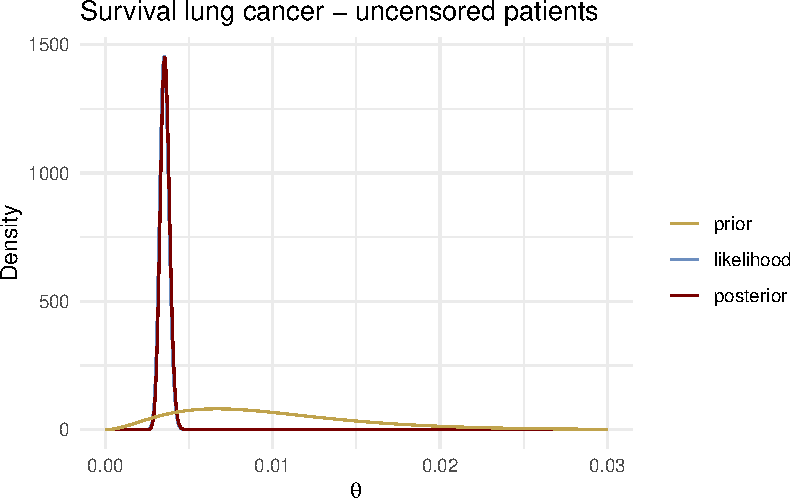
\includegraphics[keepaspectratio]{ch2solutions_files/figure-pdf/unnamed-chunk-5-1.pdf}}

\end{tcolorbox}

\begin{center}\rule{0.5\linewidth}{0.5pt}\end{center}

\subsubsection{Exercise 2.3}\label{exercise-2.3}

Let
\(X_1,\ldots,X_n \vert \theta \overset{\mathrm{iid}}{\sim} \mathrm{Geom}(\theta)\)
be iid from a geometric distribution with parameter \(0<\theta<1\). Show
that the Beta distribution is the conjugate prior for this model.

\begin{tcolorbox}[enhanced jigsaw, coltitle=black, breakable, colbacktitle=quarto-callout-note-color!10!white, colframe=quarto-callout-note-color-frame, bottomrule=.15mm, toprule=.15mm, rightrule=.15mm, arc=.35mm, colback=white, opacityback=0, bottomtitle=1mm, leftrule=.75mm, title={Solution}, titlerule=0mm, toptitle=1mm, left=2mm, opacitybacktitle=0.6]

The geometric distribution has probability mass function \[
p(x) = (1-\theta)^{x}\theta, \quad \text{ for }x=0,1,2,...
\] The likelihood from a sample of \(n\) observations is therefore \[
p(x_{1},\ldots,x_{n}\vert\theta) = \prod_{i=1}^n p(x_i \vert \theta)= (1-\theta)^{\sum_{i=1}^n x_i}\theta^{n}
\] The posterior distribution when using a
\(\theta \sim \mathrm{Beta}(\alpha,\beta)\) prior is then by Bayes'
theorem \[
p(\theta\vert x_{1},\ldots,x_n) \propto 
(1-\theta)^{\sum_{i=1}^n x_i} \theta^{n} \cdot \theta^{\alpha-1}(1-\theta)^{\beta-1}
=\theta^{\alpha + n-1}(1-\theta)^{\beta + \sum_{i=1}^n x_i-1}
\] which is proportional to the
\(\mathrm{Beta}(\alpha+n,\beta+\sum_{i=1}^n x_i)\) distribution. Since
the posterior is in the same Beta family as the prior, the prior
\(\theta \sim \mathrm{Beta}(\alpha,\beta)\) is a conjugate prior to the
geometric model.

\end{tcolorbox}

\begin{center}\rule{0.5\linewidth}{0.5pt}\end{center}

\subsubsection{Exercise 2.4}\label{exercise-2.4}

Let \(X_1,\ldots,X_n\) be an iid sample from a distribution with density
function \[
p(x) \propto \theta^2 x \exp (-x\theta)\quad \text{ for } x>0 \text{ and } \theta>0. 
\] Find the conjugate prior for this distribution and derive the
posterior distribution from an iid sample \(x_1,\ldots,x_n\).

\begin{tcolorbox}[enhanced jigsaw, coltitle=black, breakable, colbacktitle=quarto-callout-note-color!10!white, colframe=quarto-callout-note-color-frame, bottomrule=.15mm, toprule=.15mm, rightrule=.15mm, arc=.35mm, colback=white, opacityback=0, bottomtitle=1mm, leftrule=.75mm, title={Solution}, titlerule=0mm, toptitle=1mm, left=2mm, opacitybacktitle=0.6]

The likelihood function from a sample \(x_1,\ldots,x_n\) is

\[
p(x_1,\ldots,x_n \vert \theta) = \prod_{i=1}^n\theta^2 x_i \exp (-x_i\theta) \propto \theta^{2n}\exp\Big(-\theta \sum_{i=1}^n x_i \Big)
\]

This likelihood resembles a Gamma distribution, so a good guess for a
conjugate prior would be the
\(\theta \sim \mathrm{Gamma}(\alpha,\beta)\) distribution; to see that
this is indeed a reasonable guess, note that the particular form of the
Gamma density (a power of \(\theta\) times an exponential in \(\theta\))
makes it closed under multiplication. The posterior distribution is then

\[
\begin{align}
p(\theta|x_1,\ldots,x_n) & \propto p(x_1,\ldots,x_n \vert \theta)p(\theta) \\
      & \propto \theta^{2n}\exp\Big(-\theta \sum_{i=1}^n x_i \Big)\theta^{\alpha-1}\exp(-\theta\beta) \\
      & \propto \theta^{\alpha + 2n - 1}\exp\Big(-\theta (\beta+\sum_{i=1}^n x_i) \Big)
\end{align}
\] and the posterior is therefore
\(\theta \vert x_1,\ldots,x_n \sim \mathrm{Gamma}(\alpha + 2n,\beta + \sum_{i=1}^n x_i)\).
Since the posterior belongs to the same (Gamma) family as the prior, the
Gamma prior is indeed conjugate to this likelihood.

\end{tcolorbox}

\begin{center}\rule{0.5\linewidth}{0.5pt}\end{center}

\subsubsection{Exercise 2.5}\label{exercise-2.5}

\textbf{a)} Let \(x_{1},\ldots,x_{10}\) be a sample with mean
\(\bar{x}=1.873\). Assume the model
\(X_1,\ldots,X_n \overset{\mathrm{iid}}{\sim} N(\theta,1)\). Use the
prior \(\theta \sim N(0,5)\). Note that the second parameter of the
normal distribution is a variance, not a standard deviation. Compute the
posterior distribution of \(\theta\).

\begin{tcolorbox}[enhanced jigsaw, coltitle=black, breakable, colbacktitle=quarto-callout-note-color!10!white, colframe=quarto-callout-note-color-frame, bottomrule=.15mm, toprule=.15mm, rightrule=.15mm, arc=.35mm, colback=white, opacityback=0, bottomtitle=1mm, leftrule=.75mm, title={Solution}, titlerule=0mm, toptitle=1mm, left=2mm, opacitybacktitle=0.6]

We have \(n=10,\bar{x}=1.873,\sigma^{2}=1,\mu_{0}=0,\tau_{0}^{2}=5\).
The posterior is normal with \begin{align*}
      w &= \frac{\frac{10}{1}}{\frac{10}{1}+\frac{1}{5}}=\frac{50}{51}\approx0.98039 \\
      \mu_{n}   &= \frac{50}{51}\cdot1.873+\frac{1}{51}\cdot0=1.8363 \\
      \tau_{n}^{2}  &= \left(\frac{10}{1}+\frac{1}{5}\right)^{-1}=\frac{5}{51}.
    \end{align*}

\end{tcolorbox}

\textbf{b)} You now get hold of a second sample
\(Y_1,\ldots,Y_{10} | \theta \overset{\mathrm{iid}}{\sim} N(\theta ,2)\),
where \(\theta\) is the same quantity as in (a) but the measurements
have a larger variance. The sample mean in this second sample is
\(\bar{y}=0.582\). Compute the posterior distribution of \(\theta\)
using both samples (the \(x\)'s and the \(y\)'s) under the assumption
that the two samples are independent.

\(\textit{Hint}\): batch learning.

\begin{tcolorbox}[enhanced jigsaw, coltitle=black, breakable, colbacktitle=quarto-callout-note-color!10!white, colframe=quarto-callout-note-color-frame, bottomrule=.15mm, toprule=.15mm, rightrule=.15mm, arc=.35mm, colback=white, opacityback=0, bottomtitle=1mm, leftrule=.75mm, title={Solution}, titlerule=0mm, toptitle=1mm, left=2mm, opacitybacktitle=0.6]

The easiest way to do this is use the posterior from the first sample as
a prior for the second sample. That is, for this second sample we use
the prior \begin{equation*}
      \theta\sim N\left(1.836,\frac{5}{51}\right),
    \end{equation*} which gives the posterior \begin{align*}
      w &= \frac{\frac{10}{2}}{\frac{10}{2}+\frac{1}{5/51}}=\frac{25}{76} \\
\mu_{n} &= \frac{25}{76}\cdot0.582+\left(1-\frac{25}{76}\right)\cdot1.836=1.4237\\ 
\tau_{n}^{2}    &= \left(\frac{10}{2}+\frac{5}{51}\right)^{-1}=\frac{5}{76}.
    \end{align*}

\end{tcolorbox}

\textbf{c)} You finally obtain a third sample
\(Z_{1},\ldots,Z_{10} | \theta \overset{\mathrm{iid}}{\sim} N(\theta,3)\),
with mean \(\bar{z}=1.221\). Unfortunately, the measuring device for
this latter sample was defective and any measurement above \(3\) was
recorded as exactly \(3\). There were two such measurements. Give an
expression for the unnormalized posterior distribution (likelihood times
prior) for \(\theta\) based on all three samples (\(x,y\) and \(z\)).
Plot this unnormalized posterior over a grid of \(\theta\) values.

\(\textit{Hint}\): the posterior distribution is not normal anymore when
the measurements are truncated at \(3\).

\begin{tcolorbox}[enhanced jigsaw, coltitle=black, breakable, colbacktitle=quarto-callout-note-color!10!white, colframe=quarto-callout-note-color-frame, bottomrule=.15mm, toprule=.15mm, rightrule=.15mm, arc=.35mm, colback=white, opacityback=0, bottomtitle=1mm, leftrule=.75mm, title={Solution}, titlerule=0mm, toptitle=1mm, left=2mm, opacitybacktitle=0.6]

Let us do as before, using the posterior from the first two samples
(obtained in problem b) above) as the prior. The prior is therefore
\(\theta\sim N\left(1.4237,\frac{5}{76}\right)\).

Let us first use these eight observations to update the posterior, and
then add the information from the two measurements that where truncated
at \(3\). The mean of the eight measurements which were correctly
recorded is \(1.221\cdot10-3\cdot2=0.77625\). The eight correctly
recorded observations gives the following updating of the
\(N\left(1.4237,\frac{5}{76}\right)\) prior: \begin{align*}
      w &=\frac{\frac{8}{3}}{\frac{8}{3}+\frac{1}{5/76}}=\frac{10}{67} \\
      \mu_{n}   &=\frac{10}{67}\cdot0.77625+\left(1-\frac{10}{67}\right)\cdot1.4237=1.3271 \\
      \tau_{n}^{2} &=\left(\frac{8}{3}+\frac{1}{5/76}\right)^{-1}=\frac{15}{268}=0.05597.
    \end{align*} Note that most of the weight is now given to the prior,
i.e.~the posterior after the updates in (a) and (b). This is reasonable
since the \(8\) new observations have relatively large variance,
\(\sigma^{2}=3\).

We are now ready for the final piece of information: the two truncated
observations. We do not know their exact values, but we \textbf{do} know
that they were equal to or larger than \(3\). This is important
information which we cannot ignore. The likelihood of these two
observations (let's call them \(z_{1}\) and \(z_{2}\)) is \begin{align*}
      p(z_{1},z_{2}\vert\theta) &=\mathrm{Pr}(z_{1}\geq3\vert\theta)\mathrm{Pr}(z_{2}\geq3\vert\theta) \\
      &=\Big(1-\mathrm{Pr}(z_{1}\leq 3\vert\theta)\Big) \Big(1-\mathrm{Pr}(z_{2}\leq3\vert\theta)\Big) \\
      &=\left[1-\Phi\left(\frac{3-\theta}{\sqrt{3}}\right)\right]\left[1-\Phi\left(\frac{3-\theta}{\sqrt{3}}\right)\right]  \\
      &=\left[1-\Phi\left(\frac{3-\mu}{\sqrt{3}}\right)\right]^{2}
    \end{align*} where \(\Phi(\cdot)\) is the CDF of the
\(\mathrm{N}(0,1)\) distribution. The posterior based on all \(30\) data
points is now obtained by multiplying this likelihood with the prior at
this stage, that is the posterior based on the first \(28\) correctly
recorded data: \(N(1.3271,0.05597)\). The posterior is therefore
proportional to \begin{equation*}
      \left[1-\Phi\left(\frac{3-\mu}{\sqrt{3}}\right)\right]^{2}\exp\left[-\frac{1}{2\cdot0.05597}\left(\mu-1.3271\right)^{2}\right].
    \end{equation*}

The code below plots the prior (which is the posterior based on the
\(28\) correctly recorded observations), the likelihood from the two
truncated observations and the posterior based on all \(30\) data
points. Note the form of the likelihood function from the two truncated
observations: the probability of observing them increases monotonically
with \(\theta\) since all we know about these observations is that they
are larger or equal to \(3\).

\begin{Shaded}
\begin{Highlighting}[]
\NormalTok{theta\_grid }\OtherTok{=} \FunctionTok{seq}\NormalTok{(}\FloatTok{0.5}\NormalTok{, }\FloatTok{2.5}\NormalTok{, }\AttributeTok{length =} \DecValTok{1000}\NormalTok{)}
\NormalTok{bin\_width }\OtherTok{=}\NormalTok{ theta\_grid[}\DecValTok{2}\NormalTok{] }\SpecialCharTok{{-}}\NormalTok{ theta\_grid[}\DecValTok{1}\NormalTok{]}
\NormalTok{like }\OtherTok{=}\NormalTok{ (}\DecValTok{1} \SpecialCharTok{{-}} \FunctionTok{pnorm}\NormalTok{(}\DecValTok{3}\NormalTok{, theta\_grid, }\FunctionTok{sqrt}\NormalTok{(}\DecValTok{3}\NormalTok{)))}\SpecialCharTok{\^{}}\DecValTok{2} 
\NormalTok{prior }\OtherTok{=} \FunctionTok{dnorm}\NormalTok{(theta\_grid, }\FloatTok{1.3271}\NormalTok{, }\FunctionTok{sqrt}\NormalTok{(}\FloatTok{0.05597}\NormalTok{))}
\NormalTok{post }\OtherTok{=}\NormalTok{ like }\SpecialCharTok{*}\NormalTok{ prior }\CommentTok{\# unnormalized}
\NormalTok{post }\OtherTok{=}\NormalTok{ post }\SpecialCharTok{/} \FunctionTok{sum}\NormalTok{(post }\SpecialCharTok{*}\NormalTok{ bin\_width)}
\NormalTok{like }\OtherTok{=}\NormalTok{ like }\SpecialCharTok{/} \FunctionTok{sum}\NormalTok{(like }\SpecialCharTok{*}\NormalTok{ bin\_width)}
\FunctionTok{plot}\NormalTok{(theta\_grid, prior, }\AttributeTok{type =} \StringTok{"l"}\NormalTok{, }\AttributeTok{col =} \StringTok{"orange"}\NormalTok{, }\AttributeTok{lwd =} \DecValTok{3}\NormalTok{, }\AttributeTok{xlab =} \FunctionTok{expression}\NormalTok{(theta), }\AttributeTok{ylab =} \StringTok{"density"}\NormalTok{)}
\FunctionTok{lines}\NormalTok{(theta\_grid, like, }\AttributeTok{col =} \StringTok{"steelblue"}\NormalTok{, }\AttributeTok{lwd =} \DecValTok{3}\NormalTok{)}
\FunctionTok{lines}\NormalTok{(theta\_grid, post, }\AttributeTok{col =} \StringTok{"indianred"}\NormalTok{, }\AttributeTok{lwd =} \DecValTok{3}\NormalTok{)}
\FunctionTok{legend}\NormalTok{(}\StringTok{"topleft"}\NormalTok{, }\AttributeTok{legend =} \FunctionTok{c}\NormalTok{(}\StringTok{"Prior"}\NormalTok{, }\StringTok{"Likelihood"}\NormalTok{, }\StringTok{"Posterior"}\NormalTok{),}
       \AttributeTok{col =} \FunctionTok{c}\NormalTok{(}\StringTok{"orange"}\NormalTok{, }\StringTok{"steelblue"}\NormalTok{, }\StringTok{"indianred"}\NormalTok{), }\AttributeTok{lwd =} \DecValTok{3}\NormalTok{, }\AttributeTok{bty =} \StringTok{"n"}\NormalTok{)}
\end{Highlighting}
\end{Shaded}

\pandocbounded{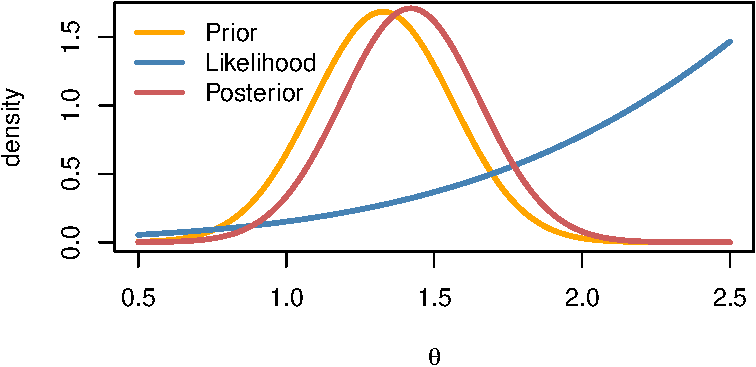
\includegraphics[keepaspectratio]{ch2solutions_files/figure-pdf/unnamed-chunk-6-1.pdf}}

\end{tcolorbox}

\begin{center}\rule{0.5\linewidth}{0.5pt}\end{center}

\subsubsection{Exercise 2.6}\label{exercise-2.6}

Derive the posterior distribution for the normal model with a normal
prior.

\emph{$\textit{Hint}$: complete the square.}

\begin{tcolorbox}[enhanced jigsaw, coltitle=black, breakable, colbacktitle=quarto-callout-note-color!10!white, colframe=quarto-callout-note-color-frame, bottomrule=.15mm, toprule=.15mm, rightrule=.15mm, arc=.35mm, colback=white, opacityback=0, bottomtitle=1mm, leftrule=.75mm, title={Solution}, titlerule=0mm, toptitle=1mm, left=2mm, opacitybacktitle=0.6]


\includegraphics[width=1.73958in,height=\textheight,keepaspectratio]{../exercises/larry.png}

\end{tcolorbox}

\begin{center}\rule{0.5\linewidth}{0.5pt}\end{center}

\subsubsection{Exercise 2.7}\label{exercise-2.7}

\textbf{a)} Let
\(X_1,\dots,X_n |\theta \sim \mathrm{Uniform}(\theta-1/2,\theta+1/2)\).
The estimator \(\hat\theta= \bar X\) is unbiased for \(\theta\).
Calculate for the sampling variance of \(\hat\theta\).

\begin{tcolorbox}[enhanced jigsaw, coltitle=black, breakable, colbacktitle=quarto-callout-note-color!10!white, colframe=quarto-callout-note-color-frame, bottomrule=.15mm, toprule=.15mm, rightrule=.15mm, arc=.35mm, colback=white, opacityback=0, bottomtitle=1mm, leftrule=.75mm, title={Solution}, titlerule=0mm, toptitle=1mm, left=2mm, opacitybacktitle=0.6]


\includegraphics[width=1.73958in,height=\textheight,keepaspectratio]{../exercises/larry.png}

\end{tcolorbox}

\textbf{b)} Derive the posterior distribution for \(\theta\) assuming a
uniform prior distribution.

\(\textit{Hint}\): once you have observed some data, some values for
\(\theta\) are no longer possible.

\begin{tcolorbox}[enhanced jigsaw, coltitle=black, breakable, colbacktitle=quarto-callout-note-color!10!white, colframe=quarto-callout-note-color-frame, bottomrule=.15mm, toprule=.15mm, rightrule=.15mm, arc=.35mm, colback=white, opacityback=0, bottomtitle=1mm, leftrule=.75mm, title={Solution}, titlerule=0mm, toptitle=1mm, left=2mm, opacitybacktitle=0.6]


\includegraphics[width=1.73958in,height=\textheight,keepaspectratio]{../exercises/larry.png}

\end{tcolorbox}

\textbf{c)} Assume that you have observed three data observations:
\(x_1 = 1.1, x_2 = 2.09, x_3 = 1.4\). What would a frequentist conclude
about \(\theta\)? What would a Bayesian conclude? Discuss.

\begin{tcolorbox}[enhanced jigsaw, coltitle=black, breakable, colbacktitle=quarto-callout-note-color!10!white, colframe=quarto-callout-note-color-frame, bottomrule=.15mm, toprule=.15mm, rightrule=.15mm, arc=.35mm, colback=white, opacityback=0, bottomtitle=1mm, leftrule=.75mm, title={Solution}, titlerule=0mm, toptitle=1mm, left=2mm, opacitybacktitle=0.6]


\includegraphics[width=1.73958in,height=\textheight,keepaspectratio]{../exercises/larry.png}

\end{tcolorbox}

\begin{center}\rule{0.5\linewidth}{0.5pt}\end{center}

\subsubsection{Exercise 2.8}\label{exercise-2.8}

Exercise \ref{ex:survival_uncens} modelled the survival times of
uncensored lung cancer patients with an iid exponential model. In this
exercise we will extend that analysis to include also the censored
patients, using the same prior as in Exercise \ref{ex:survival_uncens}.
Plot the prior and posterior densities for \(\theta\) over a suitable
grid of \(\theta\)-values. Finally, assess the fit of the exponential
model by plotting a histogram of \(\texttt{time}\) and overlay the pdf
of the exponential model with the parameter \(\theta\) estimated with
the posterior mode.

\(\textit{Hint}\): The posterior is no longer tractable due to
contributions of the censored patients to the likelihood. For the
censored patients we only know that they lived \emph{at least} the
number of days recorded in the dataset. The likelihood contribution
\(p(x_c \vert \theta)\) for the \(c\)th censored patient with recorded
time \(x_c\) is therefore
\(p(X \geq x_c \vert \theta) = e^{-\theta x_c}\), which follows from the
distribution function of the exponential distribution
\(p(X \leq x \vert \theta) = 1 - e^{-\theta x}\).

\begin{tcolorbox}[enhanced jigsaw, coltitle=black, breakable, colbacktitle=quarto-callout-note-color!10!white, colframe=quarto-callout-note-color-frame, bottomrule=.15mm, toprule=.15mm, rightrule=.15mm, arc=.35mm, colback=white, opacityback=0, bottomtitle=1mm, leftrule=.75mm, title={Solution}, titlerule=0mm, toptitle=1mm, left=2mm, opacitybacktitle=0.6]

\begin{Shaded}
\begin{Highlighting}[]
\FunctionTok{library}\NormalTok{(tidyverse) }\CommentTok{\# loads data manipulation and visualization packages}
\FunctionTok{library}\NormalTok{(survival) }\CommentTok{\# loads the lung cancer data as \textasciigrave{}lung\textasciigrave{}}
\NormalTok{colors }\OtherTok{=} \FunctionTok{c}\NormalTok{(}\StringTok{"\#6C8EBF"}\NormalTok{, }\StringTok{"\#c0a34d"}\NormalTok{, }\StringTok{"\#780000"}\NormalTok{,}\StringTok{"\#007878"}\NormalTok{,}\StringTok{"\#B5C6DF"}\NormalTok{,}\StringTok{"\#EADAAA"}\NormalTok{,}\StringTok{"\#AE6666"}\NormalTok{)}
\end{Highlighting}
\end{Shaded}

The likelihood for all data, censored and uncensored, is \[
\begin{align}
p(x_1,\ldots,x_n \vert \theta) & = \prod_{i=1}^n p(x_i \vert \theta) \\
& = \prod_{u \in \mathcal{U}} p(x_u \vert \theta) \prod_{c \in \mathcal{C}} p(x_c \vert \theta) \\
& = \prod_{u \in \mathcal{U}} p(x_u \vert \theta) \prod_{c \in \mathcal{C}} \left(1 - F(x_c \vert \theta)\right) 
\end{align}
\] where \(\mathcal{U}\) and \(\mathcal{C}\) are the sets of observation
indicies for the uncensored and censored data, respectively. The
likelihood for the uncensored data (the first product) is the same as
before \[
\prod_{u \in \mathcal{U}} p(x_u \vert \theta) = \prod_{u \in \mathcal{U}} \theta e^{-\theta x_u} = \theta^{n_u} e^{-\theta\sum_{u \in \mathcal{U}} x_u},
\] where \(n_u\) is the number of uncensored observations. The
likelihood contribution for each observation in the censored set (the
second product) is the survival function \[
\mathrm{Pr}(X \geq x_c) = 1 - F(x_c \vert \theta),
\] where \(F(x_c \vert \theta) = 1 - e^{-x_c \theta}\) is the cumulative
distribution function of the exponential distribution evaluated at
\(x_c\).

So the likelihood function is \[
p(x_1,\ldots,x_n \vert \theta) = \theta^n e^{-\theta\sum_{u \in \mathcal{U}} x_u} \times e^{-\theta \sum_{u \in \mathcal{U}} x_c} = \theta^{n_u} e^{-\theta\sum_{i = 1}^n x_i}.
\] where one should note that \(\theta\) is raised to the number of
uncensored observations, \(n_u\) while the sum in the exponential term
includes both uncensored and censored observations.

By Bayes' theorem, the posterior distribution is again a Gamma
distribution \[
\begin{align}
p(\theta \vert x_1,\ldots,x_n) & \propto p(x_1,\ldots,x_n \vert \theta)p(\theta) \\
& \propto \theta^{n_u} e^{-\theta\sum_{i = 1}^n x_i} \times \theta^{\alpha-1}e^{-\beta\theta} \\
& = \theta^{\alpha + n_u - 1} e^{ -\theta(\beta + \sum_{i = 1}^n x_i)},
\end{align}
\] which we recognize as proportional to the following Gamma
distribution \[
\theta \vert x_1,\ldots,x_n \sim \mathrm{Gamma}(\alpha + n_u,\beta + \sum\nolimits_{i=1}^n x_i).
\]

The code below plots both:

\begin{itemize}
\tightlist
\item
  the posterior from the previous exercise (a) with only the uncensored
  data and
\item
  the posterior from with all data.
\end{itemize}

The posterior with all data is more informative and concentrates on
smaller \(\theta\) values. Since smaller \(\theta\) values correspond to
longer expected survival times, this is makes sense since the censored
patients were still alive at the end of the study.

\begin{Shaded}
\begin{Highlighting}[]
\CommentTok{\# Summarize the data needed for the posterior, grouped by \textasciigrave{}status\textasciigrave{}:}
\NormalTok{data\_summary }\OtherTok{\textless{}{-}}\NormalTok{ lung }\SpecialCharTok{\%\textgreater{}\%} \FunctionTok{group\_by}\NormalTok{(status) }\SpecialCharTok{\%\textgreater{}\%} \FunctionTok{summarize}\NormalTok{(}\AttributeTok{n =} \FunctionTok{n}\NormalTok{(), }\AttributeTok{sum\_x =} \FunctionTok{sum}\NormalTok{(time))}
\end{Highlighting}
\end{Shaded}

\begin{Shaded}
\begin{Highlighting}[]
\CommentTok{\# Set up prior hyperparameters}
\NormalTok{alpha\_prior }\OtherTok{\textless{}{-}} \DecValTok{3}   \CommentTok{\# shape parameter}
\NormalTok{beta\_prior }\OtherTok{\textless{}{-}} \DecValTok{300}  \CommentTok{\# rate parameter}

\CommentTok{\# Compute posterior hyperparameters {-} only uncensored data}
\NormalTok{alpha\_post\_u }\OtherTok{\textless{}{-}}\NormalTok{ alpha\_prior }\SpecialCharTok{+}\NormalTok{ data\_summary}\SpecialCharTok{$}\NormalTok{n[}\DecValTok{2}\NormalTok{] }\CommentTok{\# second row is uncensored data (status = 2)  }
\NormalTok{beta\_post\_u }\OtherTok{\textless{}{-}}\NormalTok{ beta\_prior }\SpecialCharTok{+}\NormalTok{ data\_summary}\SpecialCharTok{$}\NormalTok{sum\_x[}\DecValTok{2}\NormalTok{] }\CommentTok{\# sum over uncensored observations}

\CommentTok{\# Compute posterior hyperparameters {-} all data}
\NormalTok{alpha\_post\_all }\OtherTok{\textless{}{-}}\NormalTok{ alpha\_prior }\SpecialCharTok{+}\NormalTok{ data\_summary}\SpecialCharTok{$}\NormalTok{n[}\DecValTok{2}\NormalTok{] }\CommentTok{\# note: this is still n\_u }
\NormalTok{beta\_post\_all }\OtherTok{\textless{}{-}}\NormalTok{ beta\_prior }\SpecialCharTok{+} \FunctionTok{sum}\NormalTok{(data\_summary}\SpecialCharTok{$}\NormalTok{sum\_x) }\CommentTok{\# sum over all observations   }
\end{Highlighting}
\end{Shaded}

\begin{Shaded}
\begin{Highlighting}[]
\CommentTok{\# Plot the prior and the two posterior densities }
\NormalTok{thetaGrid }\OtherTok{\textless{}{-}} \FunctionTok{seq}\NormalTok{(}\DecValTok{0}\NormalTok{, }\FloatTok{0.03}\NormalTok{, }\AttributeTok{length.out =} \DecValTok{1000}\NormalTok{)}
\NormalTok{prior\_density }\OtherTok{\textless{}{-}} \FunctionTok{dgamma}\NormalTok{(thetaGrid, }\AttributeTok{shape =}\NormalTok{ alpha\_prior, }\AttributeTok{rate =}\NormalTok{ beta\_prior)}
\NormalTok{posterior\_density\_u }\OtherTok{\textless{}{-}} \FunctionTok{dgamma}\NormalTok{(thetaGrid, }\AttributeTok{shape =}\NormalTok{ alpha\_post\_u, }\AttributeTok{rate =}\NormalTok{ beta\_post\_u)}
\NormalTok{posterior\_density\_all }\OtherTok{\textless{}{-}} \FunctionTok{dgamma}\NormalTok{(thetaGrid, }\AttributeTok{shape =}\NormalTok{ alpha\_post\_all, }\AttributeTok{rate =}\NormalTok{ beta\_post\_all)}


\NormalTok{df }\OtherTok{\textless{}{-}} \FunctionTok{data.frame}\NormalTok{(}
  \AttributeTok{thetaGrid =}\NormalTok{ thetaGrid, }
  \AttributeTok{prior =}\NormalTok{ prior\_density, }
  \AttributeTok{posterior\_uncensored =}\NormalTok{ posterior\_density\_u,}
  \AttributeTok{posterior\_all =}\NormalTok{ posterior\_density\_all}
\NormalTok{)}

\NormalTok{df\_long }\OtherTok{\textless{}{-}}\NormalTok{ df }\SpecialCharTok{\%\textgreater{}\%} \FunctionTok{pivot\_longer}\NormalTok{(}\SpecialCharTok{{-}}\NormalTok{thetaGrid, }\AttributeTok{names\_to =} \StringTok{"density\_type"}\NormalTok{, }\AttributeTok{values\_to =} \StringTok{"density"}\NormalTok{)}

\FunctionTok{ggplot}\NormalTok{(df\_long) }\SpecialCharTok{+}
  \FunctionTok{aes}\NormalTok{(}\AttributeTok{x =}\NormalTok{ thetaGrid, }\AttributeTok{y =}\NormalTok{ density, }\AttributeTok{color =}\NormalTok{ density\_type) }\SpecialCharTok{+}
  \FunctionTok{geom\_line}\NormalTok{() }\SpecialCharTok{+}
  \FunctionTok{scale\_colour\_manual}\NormalTok{(}
    \AttributeTok{breaks =} \FunctionTok{c}\NormalTok{(}\StringTok{"prior"}\NormalTok{, }\StringTok{"posterior\_uncensored"}\NormalTok{, }\StringTok{"posterior\_all"}\NormalTok{), }
    \AttributeTok{values =} \FunctionTok{c}\NormalTok{(colors[}\DecValTok{2}\NormalTok{], colors[}\DecValTok{3}\NormalTok{], colors[}\DecValTok{4}\NormalTok{])) }\SpecialCharTok{+}
  \FunctionTok{labs}\NormalTok{(}\AttributeTok{title =} \StringTok{"Exercise 2.2"}\NormalTok{, }\AttributeTok{x =} \FunctionTok{expression}\NormalTok{(theta), }\AttributeTok{y =} \StringTok{"Density"}\NormalTok{, }\AttributeTok{color =} \StringTok{""}\NormalTok{) }\SpecialCharTok{+} 
  \FunctionTok{theme\_minimal}\NormalTok{()}
\end{Highlighting}
\end{Shaded}

\pandocbounded{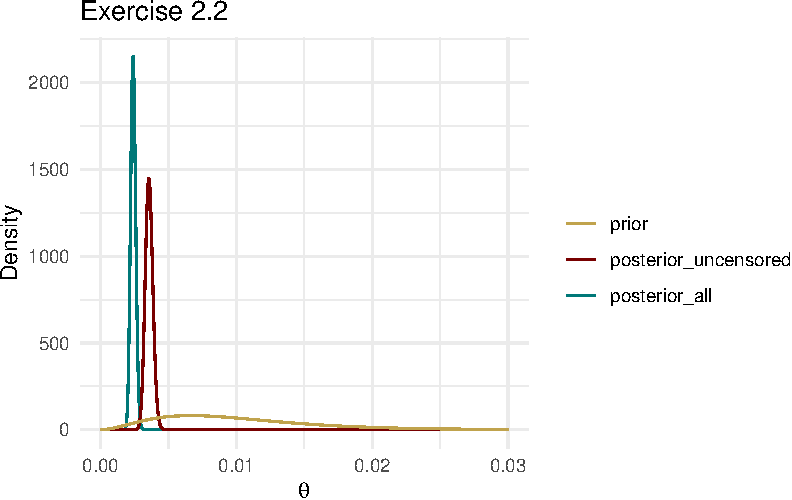
\includegraphics[keepaspectratio]{ch2solutions_files/figure-pdf/unnamed-chunk-10-1.pdf}}

The code below plots the histogram and the pdf of the exponential model
with the parameter \(\theta\) set equal to the posterior mode. It is
clear that the exponential model with its monotonically decreasing
density is not fitting the data well.

\begin{Shaded}
\begin{Highlighting}[]
\NormalTok{postMode }\OtherTok{=}\NormalTok{ df}\SpecialCharTok{$}\NormalTok{thetaGrid[}\FunctionTok{which.max}\NormalTok{(df}\SpecialCharTok{$}\NormalTok{posterior\_all)]}

\FunctionTok{ggplot}\NormalTok{(lung, }\FunctionTok{aes}\NormalTok{(time)) }\SpecialCharTok{+}
  \FunctionTok{geom\_histogram}\NormalTok{(}\FunctionTok{aes}\NormalTok{(}\AttributeTok{y =} \FunctionTok{after\_stat}\NormalTok{(density), }\AttributeTok{fill =} \StringTok{"Data"}\NormalTok{), }\AttributeTok{bins =} \DecValTok{30}\NormalTok{) }\SpecialCharTok{+}
  \FunctionTok{stat\_function}\NormalTok{(}\AttributeTok{fun =}\NormalTok{ dexp, }\AttributeTok{args =} \FunctionTok{list}\NormalTok{(}\AttributeTok{rate =}\NormalTok{ postMode), }\AttributeTok{lwd =} \DecValTok{1}\NormalTok{, }
                \FunctionTok{aes}\NormalTok{(}\AttributeTok{color =} \StringTok{"Exponential fit"}\NormalTok{),}
\NormalTok{  ) }\SpecialCharTok{+}
  \FunctionTok{labs}\NormalTok{(}\AttributeTok{title =} \StringTok{"Exercise 2.2c {-} Exponential model fit to lung cancer survival"}\NormalTok{, }\AttributeTok{x =} \StringTok{"days"}\NormalTok{, }\AttributeTok{y =} \StringTok{"Density"}\NormalTok{) }\SpecialCharTok{+} 
  \FunctionTok{scale\_fill\_manual}\NormalTok{(}\StringTok{""}\NormalTok{, }\AttributeTok{values =}\NormalTok{ colors[}\DecValTok{5}\NormalTok{]) }\SpecialCharTok{+}
  \FunctionTok{scale\_color\_manual}\NormalTok{(}\StringTok{""}\NormalTok{, }\AttributeTok{values =}\NormalTok{ colors[}\DecValTok{3}\NormalTok{]) }\SpecialCharTok{+}
  \FunctionTok{theme\_minimal}\NormalTok{()}
\end{Highlighting}
\end{Shaded}

\pandocbounded{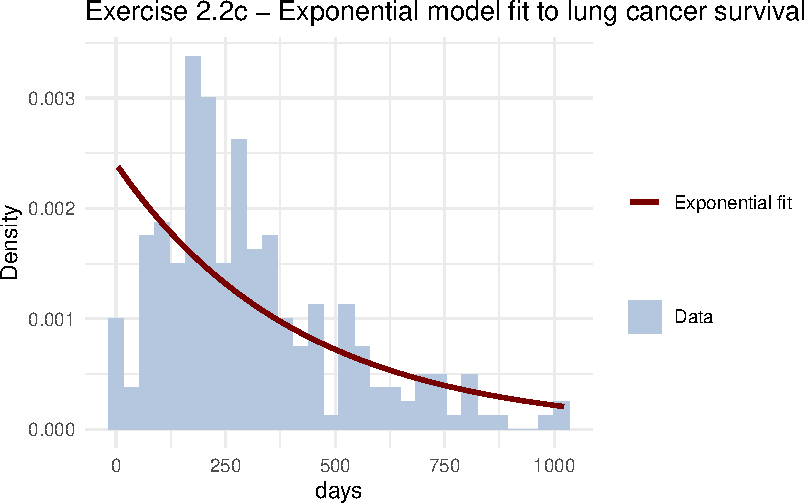
\includegraphics[keepaspectratio]{ch2solutions_files/figure-pdf/unnamed-chunk-11-1.pdf}}

\end{tcolorbox}

\begin{center}\rule{0.5\linewidth}{0.5pt}\end{center}

\subsubsection{Exercise 2.9}\label{exercise-2.9}

Show that the \(N(\mu,1)\) distribution belongs to the exponential
family.

\begin{tcolorbox}[enhanced jigsaw, coltitle=black, breakable, colbacktitle=quarto-callout-note-color!10!white, colframe=quarto-callout-note-color-frame, bottomrule=.15mm, toprule=.15mm, rightrule=.15mm, arc=.35mm, colback=white, opacityback=0, bottomtitle=1mm, leftrule=.75mm, title={Solution}, titlerule=0mm, toptitle=1mm, left=2mm, opacitybacktitle=0.6]


\includegraphics[width=1.73958in,height=\textheight,keepaspectratio]{../exercises/larry.png}

\end{tcolorbox}

\begin{center}\rule{0.5\linewidth}{0.5pt}\end{center}

\subsubsection{Exercise 2.10}\label{exercise-2.10}

Exercise \ref{ex:survival_all} modelled the survival times of uncensored
lung cancer patients with an iid exponential model. Here we extend that
analysis to the more general Weibull distribution: \[
X_1,\ldots,X_n \vert \lambda, k \overset{\mathrm{iid}}{\sim} \mathrm{Weibull}(\lambda,k).
\] The value of \(k\) determines how the failure rate changes with time:

\begin{itemize}
    \item $k=1$ gives a failure (death) rate that is constant over time and corresponds to the special case of a exponential distribution $\mathrm{Expon}(\theta=1/\lambda)$ used in Exercise 2.2. Note that (following Wikipedia) the exponential distribution is parameterized with a rate (inverse scale) parameter $\theta$, while the Weibull is parameterized with a scale parameter $\lambda= 1/\theta$
    \item $k<1$ gives a decreasing failure rate over time
    \item $k>1$ gives an increasing failure rate over time.
\end{itemize}

Plot the posterior distribution of \(\lambda\) conditional on \(k=1\),
\(k=3/2\) and \(k=2\). For all \(k\), use the prior
\(\lambda \sim \mathrm{Gamma}(\alpha,\beta)\) with \(\alpha=3\) and
\(\beta=1/50\) (which is a similar prior for \(\theta=1/\lambda\) as in
Exercise 2.2). Plot the \texttt{time} variable as a histogram and
overlay the fitted model for the three different \(k\)-values; use the
posterior mode for \(\theta\) in each model when plotting the fitted
model density.

\(\textit{Hint}\): the posterior distribution for \(k\neq 1\) is
intractable, so use numerical evaluation of the posterior over a grid of
\(\lambda\)-values.

\begin{tcolorbox}[enhanced jigsaw, coltitle=black, breakable, colbacktitle=quarto-callout-note-color!10!white, colframe=quarto-callout-note-color-frame, bottomrule=.15mm, toprule=.15mm, rightrule=.15mm, arc=.35mm, colback=white, opacityback=0, bottomtitle=1mm, leftrule=.75mm, title={Solution}, titlerule=0mm, toptitle=1mm, left=2mm, opacitybacktitle=0.6]

The likelihood can be computed with separate treatment of the uncensored
and censored observations: \[
\begin{align}
p(x_1,\ldots,x_n \vert \lambda, k) & = \prod_{i=1}^n p(x_i \vert \lambda, k) \\
& = \prod_{u \in \mathcal{U}} p(x_u \vert \lambda, k) \prod_{c \in \mathcal{C}} \Big(1 - F(x_c \vert \lambda, k)\Big) 
\end{align}
\] where \(p(x \vert \lambda, k)\) is the pdf of a Weibull variable \[
p(x \vert \lambda, k) = \frac{k}{\lambda}\Big( \frac{x}{\lambda} \Big)^{k-1}e^{-(x/\lambda)^k}\quad\text{ for }x>0
\] which is implemented in R as \texttt{dweibull}. The cdf of the
Weibull distribution is of rather simple form \[
F(x \vert \lambda, k) = 1 - e^{-(x/\lambda)^k}
\] and is implemented in R as \texttt{pweibull}.

The code below plots the prior and posterior distribution for
\(\lambda\) for the three different \(k\)-values. We could have inserted
the mathematical expressions for the pdf and cdf and simplified the
final likelihood expression; we will instead use the \texttt{dweibull}
and \texttt{pweibull} functions without simplifications since it gives a
more general template that can be used for any distribution, not just
the Weibull model. For numerical stability we usually compute the
posterior distribution on the log scale \[
\log p(\lambda^{(j)} \vert x_1,\ldots,x_n) \propto \log p(x_1,\ldots,x_n \vert \lambda_j) + \log p(\lambda_j)
\] for a grid of equally spaced \(\lambda\)-values:
\(\lambda^{(1)}\ldots,\lambda^{(J)}\). The \(\propto\) sign now means
that there is a missing \emph{additive} constant
\(\log p(x_1,\ldots,x_n)\) which does not depend on the unknown
parameter \(\lambda\). When we have computed
\(\log p(\lambda \vert x_1,\ldots,x_n)\) over a grid of \(\lambda\)
values we compute the posterior on the original scale by \[
p(\lambda^{(j)} \vert x_1,\ldots,x_n) \propto \exp\Big( \log p(x_1,\ldots,x_n \vert \lambda_j) + \log p(\lambda_j) \Big)
\] and then divide all numbers with the normalizing constant to make
sure that the posterior integrates to one. This is done numerically by
approximating the integral by a Riemann rectangle sum \[
p(\lambda^{(j)} \vert x_1,\ldots,x_n) = 
\frac{\exp\Big( \log p(x_1,\ldots,x_n \vert \lambda^{(j)}) + \log p(\lambda^{(j)}) \Big)}
{\sum_{h=1}^J \exp\Big( \log p(x_1,\ldots,x_n \vert \lambda^{(h)}) + \log p(\lambda^{(h)}) \Big) \Delta}
\] where \(\Delta\) is the spacing between the grid points of
\(\lambda\)-values: \(\lambda^{(1)}, \ldots, \lambda^{(J)}\).

\begin{Shaded}
\begin{Highlighting}[]
\FunctionTok{library}\NormalTok{(tidyverse) }\CommentTok{\# loads data manipulation and visualization packages}
\FunctionTok{library}\NormalTok{(survival) }\CommentTok{\# loads the lung cancer data as \textasciigrave{}lung\textasciigrave{}}
\NormalTok{colors }\OtherTok{=} \FunctionTok{c}\NormalTok{(}\StringTok{"\#6C8EBF"}\NormalTok{, }\StringTok{"\#c0a34d"}\NormalTok{, }\StringTok{"\#780000"}\NormalTok{,}\StringTok{"\#007878"}\NormalTok{,}\StringTok{"\#B5C6DF"}\NormalTok{,}\StringTok{"\#EADAAA"}\NormalTok{,}\StringTok{"\#AE6666"}\NormalTok{)}
\end{Highlighting}
\end{Shaded}

Set up prior hyperparameters

\begin{Shaded}
\begin{Highlighting}[]
\NormalTok{alpha\_prior }\OtherTok{\textless{}{-}} \DecValTok{3}     \CommentTok{\# shape parameter}
\NormalTok{beta\_prior }\OtherTok{\textless{}{-}} \DecValTok{1}\SpecialCharTok{/}\DecValTok{50}   \CommentTok{\# rate parameter}
\end{Highlighting}
\end{Shaded}

Set up function that computes the likelihood for any \(\lambda\) value:

\begin{Shaded}
\begin{Highlighting}[]
\CommentTok{\# Make a function that computes the likelihood}
\NormalTok{weibull\_loglike }\OtherTok{\textless{}{-}} \ControlFlowTok{function}\NormalTok{(lambda, x, censored, k)\{}
\NormalTok{  loglik\_uncensored }\OtherTok{=} \FunctionTok{sum}\NormalTok{(}\FunctionTok{dweibull}\NormalTok{(x[}\SpecialCharTok{{-}}\NormalTok{censored], }\AttributeTok{shape =}\NormalTok{ k, }\AttributeTok{scale =}\NormalTok{ lambda, }
                                   \AttributeTok{log =} \ConstantTok{TRUE}\NormalTok{))}
\NormalTok{  loglik\_censored }\OtherTok{=} \FunctionTok{sum}\NormalTok{(}\FunctionTok{pweibull}\NormalTok{(x[censored], }\AttributeTok{shape =}\NormalTok{ k, }\AttributeTok{scale =}\NormalTok{ lambda, }
                                 \AttributeTok{lower.tail =} \ConstantTok{FALSE}\NormalTok{, }\AttributeTok{log.p =} \ConstantTok{TRUE}\NormalTok{))}
  \FunctionTok{return}\NormalTok{(loglik\_uncensored }\SpecialCharTok{+}\NormalTok{ loglik\_censored)}
\NormalTok{\}}
\end{Highlighting}
\end{Shaded}

Set up a function that computes the posterior density over a grid of
\(\lambda\):

\begin{Shaded}
\begin{Highlighting}[]
\NormalTok{weibull\_posterior }\OtherTok{\textless{}{-}} \ControlFlowTok{function}\NormalTok{(lambdaGrid, x, censored, k, alpha\_prior, beta\_prior)\{}
\NormalTok{  Delta }\OtherTok{=}\NormalTok{ lambdaGrid[}\DecValTok{2}\NormalTok{] }\SpecialCharTok{{-}}\NormalTok{ lambdaGrid[}\DecValTok{1}\NormalTok{] }\CommentTok{\# Grid step size}
\NormalTok{  logPrior }\OtherTok{\textless{}{-}} \FunctionTok{dgamma}\NormalTok{(lambdaGrid, }\AttributeTok{shape =}\NormalTok{ alpha\_prior, }\AttributeTok{rate =}\NormalTok{ beta\_prior, }\AttributeTok{log =} \ConstantTok{TRUE}\NormalTok{)}
\NormalTok{  logLike }\OtherTok{\textless{}{-}} \FunctionTok{sapply}\NormalTok{(lambdaGrid, weibull\_loglike, x, censored, k)}
\NormalTok{  logPost }\OtherTok{\textless{}{-}}\NormalTok{ logLike }\SpecialCharTok{+}\NormalTok{ logPrior}
\NormalTok{  logPost }\OtherTok{\textless{}{-}}\NormalTok{ logPost }\SpecialCharTok{{-}} \FunctionTok{max}\NormalTok{(logPost) }\CommentTok{\# subtract constant to avoid overflow}
\NormalTok{  post }\OtherTok{\textless{}{-}} \FunctionTok{exp}\NormalTok{(logPost)}\SpecialCharTok{/}\NormalTok{(}\FunctionTok{sum}\NormalTok{(}\FunctionTok{exp}\NormalTok{(logPost))}\SpecialCharTok{*}\NormalTok{Delta) }\CommentTok{\# original scale and normalize}
\NormalTok{  logLike }\OtherTok{\textless{}{-}}\NormalTok{ logLike }\SpecialCharTok{{-}} \FunctionTok{max}\NormalTok{(logLike)}
\NormalTok{  likeNorm }\OtherTok{\textless{}{-}} \FunctionTok{exp}\NormalTok{(logLike)}\SpecialCharTok{/}\NormalTok{(}\FunctionTok{sum}\NormalTok{(}\FunctionTok{exp}\NormalTok{(logLike))}\SpecialCharTok{*}\NormalTok{Delta) }\CommentTok{\# normalized likelihood}
  \FunctionTok{return}\NormalTok{(}\FunctionTok{list}\NormalTok{(}\AttributeTok{post =}\NormalTok{ post, }\AttributeTok{prior =} \FunctionTok{exp}\NormalTok{(logPrior), }\AttributeTok{likeNorm =}\NormalTok{ likeNorm))}
\NormalTok{\}}
\end{Highlighting}
\end{Shaded}

\begin{Shaded}
\begin{Highlighting}[]
\CommentTok{\# Plot the prior and posterior densities}

\NormalTok{lambdaGrid }\OtherTok{\textless{}{-}} \FunctionTok{seq}\NormalTok{(}\DecValTok{200}\NormalTok{, }\DecValTok{800}\NormalTok{, }\AttributeTok{length.out =} \DecValTok{1000}\NormalTok{)}
\CommentTok{\# Compute to get the prior}
\NormalTok{postRes }\OtherTok{\textless{}{-}} \FunctionTok{weibull\_posterior}\NormalTok{(lambdaGrid, lung}\SpecialCharTok{$}\NormalTok{time, lung}\SpecialCharTok{$}\NormalTok{status }\SpecialCharTok{==} \DecValTok{1}\NormalTok{, }\AttributeTok{k =} \DecValTok{1}\NormalTok{, }
\NormalTok{                             alpha\_prior, beta\_prior)}
\NormalTok{df }\OtherTok{\textless{}{-}} \FunctionTok{data.frame}\NormalTok{(}
  \AttributeTok{lambdaGrid =}\NormalTok{ lambdaGrid, }
  \AttributeTok{prior =}\NormalTok{ postRes}\SpecialCharTok{$}\NormalTok{prior}
\NormalTok{)}

\CommentTok{\# Compute for all selected k values}
\NormalTok{postModes }\OtherTok{=} \FunctionTok{c}\NormalTok{()}
\ControlFlowTok{for}\NormalTok{ (k }\ControlFlowTok{in} \FunctionTok{c}\NormalTok{(}\DecValTok{1}\NormalTok{, }\DecValTok{3}\SpecialCharTok{/}\DecValTok{2}\NormalTok{, }\DecValTok{2}\NormalTok{))\{}
\NormalTok{  postRes }\OtherTok{\textless{}{-}} \FunctionTok{weibull\_posterior}\NormalTok{(lambdaGrid, lung}\SpecialCharTok{$}\NormalTok{time, lung}\SpecialCharTok{$}\NormalTok{status }\SpecialCharTok{==} \DecValTok{1}\NormalTok{, k, alpha\_prior, beta\_prior)}
\NormalTok{  df[}\FunctionTok{str\_glue}\NormalTok{(}\StringTok{"posterior k=\{k\}"}\NormalTok{)] }\OtherTok{\textless{}{-}}\NormalTok{ postRes}\SpecialCharTok{$}\NormalTok{post}
\NormalTok{  postModes }\OtherTok{=} \FunctionTok{c}\NormalTok{(postModes, lambdaGrid[}\FunctionTok{which.max}\NormalTok{(postRes}\SpecialCharTok{$}\NormalTok{post)])}
\NormalTok{\}}

\NormalTok{df\_long }\OtherTok{\textless{}{-}}\NormalTok{ df }\SpecialCharTok{\%\textgreater{}\%} \FunctionTok{pivot\_longer}\NormalTok{(}\SpecialCharTok{{-}}\NormalTok{lambdaGrid, }\AttributeTok{names\_to =} \StringTok{"density\_type"}\NormalTok{, }\AttributeTok{values\_to =} \StringTok{"density"}\NormalTok{)}

\CommentTok{\# Plot using ggplot2}
\FunctionTok{ggplot}\NormalTok{(df\_long) }\SpecialCharTok{+}
  \FunctionTok{aes}\NormalTok{(}\AttributeTok{x =}\NormalTok{ lambdaGrid, }\AttributeTok{y =}\NormalTok{ density, }\AttributeTok{color =}\NormalTok{ density\_type) }\SpecialCharTok{+}
  \FunctionTok{geom\_line}\NormalTok{() }\SpecialCharTok{+}
  \FunctionTok{xlim}\NormalTok{(}\DecValTok{250}\NormalTok{,}\DecValTok{600}\NormalTok{) }\SpecialCharTok{+}
  \FunctionTok{scale\_colour\_manual}\NormalTok{(}
    \AttributeTok{breaks =} \FunctionTok{c}\NormalTok{(}\StringTok{"prior"}\NormalTok{, }\StringTok{"posterior k=1"}\NormalTok{, }\StringTok{"posterior k=1.5"}\NormalTok{, }\StringTok{"posterior k=2"}\NormalTok{), }
    \AttributeTok{values =} \FunctionTok{c}\NormalTok{(colors[}\DecValTok{2}\NormalTok{], colors[}\DecValTok{1}\NormalTok{], colors[}\DecValTok{3}\NormalTok{], colors[}\DecValTok{4}\NormalTok{])) }\SpecialCharTok{+}
  \FunctionTok{labs}\NormalTok{(}\AttributeTok{title =} \StringTok{"Exercise 2.3"}\NormalTok{, }\AttributeTok{x =} \FunctionTok{expression}\NormalTok{(lambda), }\AttributeTok{y =} \StringTok{"Density"}\NormalTok{, }\AttributeTok{color =} \StringTok{""}\NormalTok{) }\SpecialCharTok{+} 
  \FunctionTok{theme\_minimal}\NormalTok{()}
\end{Highlighting}
\end{Shaded}

\begin{verbatim}
Warning: Removed 1668 rows containing missing values or values outside the scale range
(`geom_line()`).
\end{verbatim}

\pandocbounded{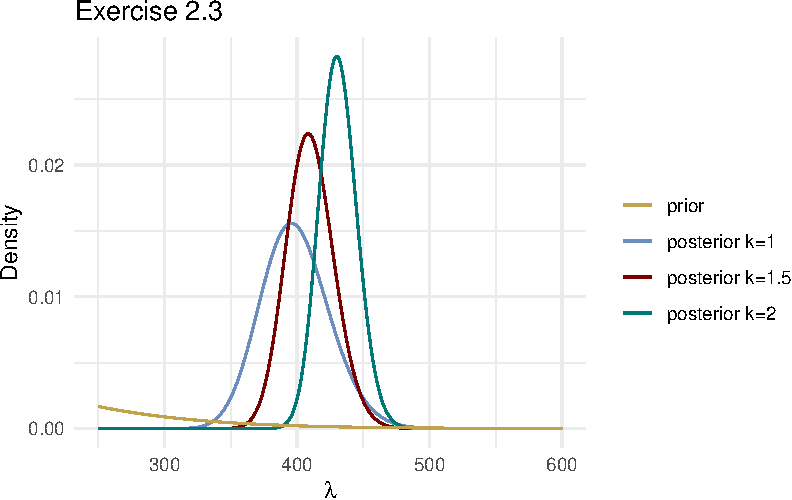
\includegraphics[keepaspectratio]{ch2solutions_files/figure-pdf/unnamed-chunk-16-1.pdf}}

The fit of the three Weibull models are plotted below. The best fit
seems to be for \(k=3/2\), but it is still not very good. In a later
exercise you will be asked to freely estimate both \(\lambda\) and
\(k\), and even later to fit a Weibull regression model with covariates.

\begin{Shaded}
\begin{Highlighting}[]
\FunctionTok{ggplot}\NormalTok{(lung, }\FunctionTok{aes}\NormalTok{(time)) }\SpecialCharTok{+}
  \FunctionTok{geom\_histogram}\NormalTok{(}\FunctionTok{aes}\NormalTok{(}\AttributeTok{y =} \FunctionTok{after\_stat}\NormalTok{(density), }\AttributeTok{fill =} \StringTok{"Data"}\NormalTok{), }\AttributeTok{bins =} \DecValTok{30}\NormalTok{) }\SpecialCharTok{+}
  \FunctionTok{stat\_function}\NormalTok{(}\AttributeTok{fun =}\NormalTok{ dweibull, }\AttributeTok{args =} \FunctionTok{list}\NormalTok{(}\AttributeTok{shape =} \DecValTok{1}\NormalTok{, }\AttributeTok{scale =}\NormalTok{ postModes[}\DecValTok{1}\NormalTok{]), }\AttributeTok{lwd =} \DecValTok{1}\NormalTok{, }
                \FunctionTok{aes}\NormalTok{(}\AttributeTok{color =} \StringTok{"Weibull fit k = 1"}\NormalTok{),}
\NormalTok{  ) }\SpecialCharTok{+}
  \FunctionTok{stat\_function}\NormalTok{(}\AttributeTok{fun =}\NormalTok{ dweibull, }\AttributeTok{args =} \FunctionTok{list}\NormalTok{(}\AttributeTok{shape =} \DecValTok{3}\SpecialCharTok{/}\DecValTok{2}\NormalTok{, }\AttributeTok{scale =}\NormalTok{ postModes[}\DecValTok{2}\NormalTok{]), }\AttributeTok{lwd =} \DecValTok{1}\NormalTok{, }
                \FunctionTok{aes}\NormalTok{(}\AttributeTok{color =} \StringTok{"Weibull fit k = 3/2"}\NormalTok{),}
\NormalTok{  ) }\SpecialCharTok{+}
  \FunctionTok{stat\_function}\NormalTok{(}\AttributeTok{fun =}\NormalTok{ dweibull, }\AttributeTok{args =} \FunctionTok{list}\NormalTok{(}\AttributeTok{shape =} \DecValTok{2}\NormalTok{, }\AttributeTok{scale =}\NormalTok{ postModes[}\DecValTok{3}\NormalTok{]), }\AttributeTok{lwd =} \DecValTok{1}\NormalTok{, }
                \FunctionTok{aes}\NormalTok{(}\AttributeTok{color =} \StringTok{"Weibull fit k = 2"}\NormalTok{),}
\NormalTok{  ) }\SpecialCharTok{+}
  \FunctionTok{labs}\NormalTok{(}\AttributeTok{title =} \StringTok{"Weibull model fits"}\NormalTok{, }\AttributeTok{x =} \StringTok{"days"}\NormalTok{, }\AttributeTok{y =} \StringTok{"Density"}\NormalTok{) }\SpecialCharTok{+} 
  \FunctionTok{scale\_fill\_manual}\NormalTok{(}\StringTok{""}\NormalTok{, }\AttributeTok{values =}\NormalTok{ colors[}\DecValTok{6}\NormalTok{]) }\SpecialCharTok{+}
  \FunctionTok{scale\_color\_manual}\NormalTok{(}\StringTok{""}\NormalTok{, }\AttributeTok{values =} \FunctionTok{c}\NormalTok{(colors[}\DecValTok{1}\NormalTok{], colors[}\DecValTok{3}\NormalTok{], colors[}\DecValTok{4}\NormalTok{])) }\SpecialCharTok{+}
  \FunctionTok{theme\_minimal}\NormalTok{()}
\end{Highlighting}
\end{Shaded}

\pandocbounded{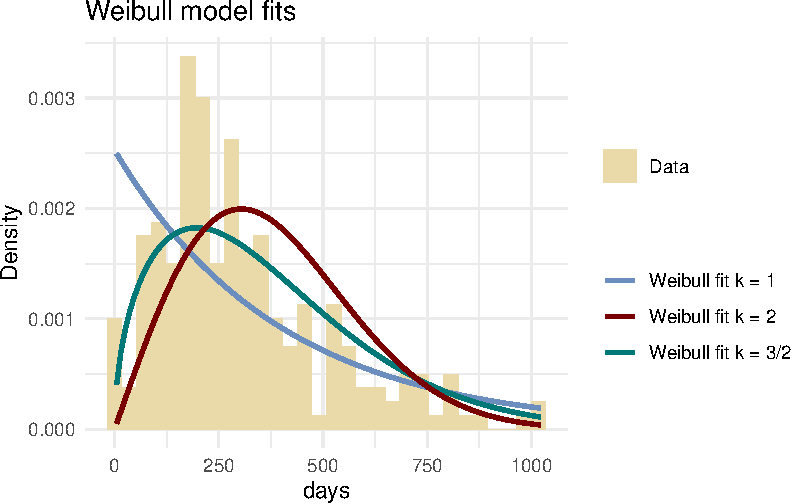
\includegraphics[keepaspectratio]{ch2solutions_files/figure-pdf/unnamed-chunk-17-1.pdf}}

\end{tcolorbox}

\begin{center}\rule{0.5\linewidth}{0.5pt}\end{center}

\subsubsection{Exercise 2.11}\label{exercise-2.11}

Let \[
X_1,\ldots,X_n \overset{iid}{\sim } \mathrm{Uniform}(0,\theta).
\] Show that the Pareto prior
\(\theta \sim \mathrm{Pareto}(\alpha, \beta)\), is conjugate to the
Uniform model by deriving the posterior distribution. See
Box\textasciitilde{}\ref{box:paretodistproperties} for a definition of
the Pareto distribution and properties; note the support of the Pareto
distribution.

\(\textit{Hint}\): Do not forget to include an indicator function when
you write up the likelihood function since the
\(\mathrm{Uniform}(0,\theta)\) distribution is zero for outcomes larger
than \(\theta\).

\begin{tcolorbox}[enhanced jigsaw, coltitle=black, breakable, colbacktitle=quarto-callout-note-color!10!white, colframe=quarto-callout-note-color-frame, bottomrule=.15mm, toprule=.15mm, rightrule=.15mm, arc=.35mm, colback=white, opacityback=0, bottomtitle=1mm, leftrule=.75mm, title={Solution}, titlerule=0mm, toptitle=1mm, left=2mm, opacitybacktitle=0.6]

The pdf of the \(\mathrm{Uniform}(0,\theta)\) distribution is
\begin{equation*}
  p(x) = \begin{cases}
          \frac{1}{\theta}  & \text{if } x \leq  \theta \\
          0                 & \text{otherwise }
          \end{cases}
\end{equation*} which can be written with an indicator function as \[
p(x) = \frac{1}{\theta} I(x_i \leq \theta).
\] The likelihood function is therefore of the form \begin{equation*}
   p(x_1,\ldots,x_n\vert\theta) = \prod_{i=1}^n \frac{1}{\theta} I(x_i \leq \theta) = \frac{1}{\theta^n} \prod_{i=1}^n I(x_i \leq \theta).
\end{equation*} The factor \(\prod_{i=1}^n I(x_i \leq \theta)\) is only
non-zero if \emph{all} \(x_1,\ldots,x_n\) are smaller or equal to
\(\theta\), i.e.~if \(x_{\mathrm{max}} := \mathrm{max}(x_1, \dots,x_n)\)
is smaller or equal to \(\theta\). We can therefore write the likelihood
as \begin{equation*}
   p(x_1,\ldots,x_n\vert\theta) = \frac{1}{\theta^n}  I(x_{\mathrm{max}} \leq \theta).
\end{equation*}

The Pareto prior can also be written with an indicator function
\begin{align*}
    p(\theta) = \frac{\alpha \beta^\alpha }{\theta^{\alpha+1}}\cdot I(\beta \leq \theta),
\end{align*} to explicitly include that \(p(\theta)=0\) if
\(\theta < \beta\).

By Bayes' theorem, the posterior is then \begin{align*}
    p(\theta \vert x_1, \dots,x_n) &\propto p(x_1, \dots,x_n \vert \theta)p(\theta) \\
                       &= \frac{1}{\theta^n} I(x_{\mathrm{max}} \leq \theta)
                            \frac{\alpha \beta^\alpha }{\theta^{\alpha+1}}\cdot I(\beta \leq \theta) \\
                       &=  \frac{\alpha \beta^\alpha }{\theta^{n+\alpha+1}} \cdot  
                            I\big(\tilde \beta \leq \theta \big)        
\end{align*} where
\(\tilde \beta = \mathrm{max}(x_{\mathrm{max}},\beta)\). This is
proportional to a \(\mathrm{Pareto}\big(\alpha + n, \tilde \beta \big)\)
density. Since the prior and posterior are both in the Pareto family,
the Pareto prior is conjugate to the \(\mathrm{Uniform}(0,\theta)\)
model.

\end{tcolorbox}




\end{document}
